% CS F407 Artificial Intelligence: final project report template.
% Limit: 2 pages, including everything except references.
% Do not change the font size, margins or spacing.
\documentclass[11pt,a4paper,twocolumn]{article}

\usepackage[margin=2cm,columnsep=0.8cm]{geometry}
\usepackage[T1]{fontenc}
\usepackage{lmodern}
\usepackage{microtype}
\usepackage{amsmath,amssymb}
\usepackage{graphicx}
\usepackage{booktabs}
\usepackage{tabularx}
\usepackage{enumitem}
\usepackage{titlesec}
\usepackage[hidelinks]{hyperref}

\titleformat{\section}{\normalsize\bfseries}{\thesection}{0.6em}{}
\titlespacing*{\section}{0pt}{1.2ex plus 0.3ex}{0.6ex}
\setlist{nosep,leftmargin=*}
\setlength{\parskip}{0.3ex}

\newcommand{\coursename}{CS F407 Artificial Intelligence, AY 2026--27 Semester I}
\newcommand{\teamno}{Team XX}
\newcommand{\githuburl}{https://github.com/meemansa-jha/indus-epigraphy}

\begin{document}

\twocolumn[{%
\begin{center}
  {\large\bfseries Confidence Is Not Understanding: An Indus Script Parsing Engine\\with Guardrails Against Semantic Hallucination}\\[1ex]
  \teamno\\
  Member One (2022A7PS0001G), Member Two (2022A7PS0002G), Member Three (2022A7PS0003G)\\[0.5ex]
  {\small \coursename, BITS Pilani, K.K. Birla Goa Campus}\\[1.5ex]
  \begin{minipage}{0.85\textwidth}
    \small
    \centerline{\bfseries Abstract}\vspace{0.5ex}
    The Indus script is undeciphered, yet AI systems readily produce confident outputs about it. We built
    a four-stage engine that reads sign sequences from images (YOLOv8 + MobileNetV3), models positional
    statistics with smoothed Markov chains, restores damaged signs with a calibrated masked Transformer,
    and checks every output against structural controls (shuffled, random and Markov-generated
    inscriptions). Positional findings are robust: the reading direction and a dominant text-final sign
    replicate on a corpus 20 times larger (flip test $p<10^{-4}$). The masked model restores 33.3\% of
    hidden signs in 5-fold cross-validation, slightly but significantly better than a Witten--Bell bigram
    (32.5\%, McNemar $p=0.008$). Vision scores 88\% top-1 on synthetic images but 12--17\% on real seals,
    and our guardrail rejects 74\% of those real readings. The guardrail cannot separate Markov fakes from
    real text, and the model is ``highly confident'' on 8--10\% of pure noise: statistical plausibility
    must not be mistaken for meaning.
  \end{minipage}
\end{center}
\vspace{1.5ex}
}]

\section{Introduction}
About 4,000 Indus inscriptions survive, averaging five signs each; there is no bilingual text and no
accepted decipherment~\cite{mahadevan1977,wells2015}. Models fitted to sign sequences still produce fluent, confident outputs (completions, ``readings'',
generated texts) that are easy to mistake for understanding. Our question is therefore not ``what do the inscriptions
say?'' but ``which computational claims about them survive a control that removes the language?''

\textbf{Input and output.} The engine takes either a photograph of an inscription strip or a typed sign
sequence (in any of three sign numberings), and outputs (i)~the sign sequence in reading order,
(ii)~positional $n$-gram probabilities for every transition, (iii)~for every sign, the probability a
masked model assigns to it and its top alternatives, and (iv)~a verdict on whether the sequence is
statistically consistent with real inscriptions.

\textbf{Contributions.} (1)~A reproducible four-stage pipeline with a validated crosswalk between three
sign numberings; (2)~positional findings replicated on two corpora and a published table; (3)~a
calibrated masked-sign model tested against statistical baselines; (4)~a benchmark that tests every
claim, including a proposed reading and our own generated texts, against structural controls.

\section{Background and related work}
\textbf{Indus statistics.} Rao et al.~\cite{rao2009} argued from conditional entropy that the script
behaves like language; Yadav et al.~\cite{yadav2010} reported strong positional regularities; Farmer
et al.~\cite{farmer2004} and Sproat~\cite{sproat2014} showed that such statistics do not distinguish
language from non-linguistic symbol systems. We adopt their standard: a statistic is evidence only if it
beats a matched control. \textbf{Vision.} Dixit et al.~\cite{dixit2025} detect and
classify 40 sign classes with YOLOv3 and MobileNet using 232 hand-annotated seals; their data are
available only on request. \textbf{Techniques.} We use Witten--Bell smoothing for sparse
$n$-grams~\cite{wittenbell1991}, a BERT-style masked encoder~\cite{devlin2019} scored by
pseudo-perplexity~\cite{salazar2020}, temperature calibration~\cite{guo2017}, YOLOv8~\cite{yolov8} and
MobileNetV3~\cite{howard2019}, and compare embeddings from word2vec~\cite{mikolov2013} and
LLM2Vec~\cite{llm2vec2024} (both suggested by faculty) with Naive Bayes classifiers as guardrails
~\cite{russell2021aima}.

\section{Method}
\textbf{Data and sign numbering.} Three numberings are in use: Mahadevan's IM77~\cite{mahadevan1977}
(417 sign templates~\cite{im417}), Parpola's (CISI corpus~\cite{cisi1987}, 179 inscriptions) and Wells'
(a CSV of 5,679 transcriptions~\cite{csvsource}). We built a crosswalk from the CISI sign records; it
maps 334 of 417 IM77 signs and agrees with independent transcriptions on 91.8\% of 785 shared sign
slots. Both corpora are stored left-to-right; the script reads right-to-left, so all sequences are
reversed before positional analysis.

\textbf{M1: vision.} The only sign image set has one template per sign, and no labelled real
photographs exist. We therefore render templates as carved relief under random lighting, wear, blur and
perspective (2,500 synthetic strips; 41,700 single-sign crops), train a single-class YOLOv8n detector and
a 417-way MobileNetV3-Small recognizer, and order boxes right-to-left.

\textbf{M2: positional statistics.} We measure start/end asymmetry with a flip test (Jensen--Shannon
divergence between first- and last-sign distributions vs.\ randomly flipped texts), position entropies,
and a reading-order bigram with Witten--Bell smoothing,
\begin{equation}
P(b\mid a)=\frac{c(a,b)+t(a)\,P_{\text{uni}}(b)}{c(a)+t(a)},
\end{equation}
where $t(a)$ is the number of distinct successors of $a$. Collocations are pairs with $c\ge3$ and
Benjamini--Hochberg-corrected Fisher $q<0.05$.

\textbf{M3: masked-sign model.} A Transformer encoder (2 layers, $d{=}64$, 4 heads, chosen by
validation search over 5 configurations) is trained to predict masked signs. Three seeds form an
ensemble whose probabilities are temperature-scaled ($T{=}1.15$) on validation data. An inscription
$x_{1..n}$ is scored by pseudo-perplexity
\begin{equation}
\mathrm{PPPL}(x)=\exp\!\Big(-\tfrac{1}{n}\textstyle\sum_{i=1}^{n}\log p(x_i\mid x_{\setminus i})\Big).
\end{equation}

\textbf{M4: controls and guardrails.} For every real test inscription we create four controls: shuffled
(same signs, random order), frequency-random and uniform-random (same length), and Markov-generated
(sampled from the bigram). The \emph{perplexity guardrail} flags $x$ if $\mathrm{PPPL}(x)>\tau$, with
$\tau=597$ the 95th percentile on real validation texts. A multinomial \emph{Naive Bayes guardrail} on
sign unigrams and bigrams is trained to separate real texts from each control.

\textbf{Engine and generation.} The engine chains M1 $\rightarrow$ crosswalk $\rightarrow$ M2
$\rightarrow$ M3 $\rightarrow$ M4 (Fig.~\ref{fig:engine}) and labels whether input was typed or read
automatically. New inscriptions are generated by Markov sampling and by Gibbs sampling from M3 (10
sweeps of resampling each sign given the rest); outputs that copy, or are one edit away from, a training
text are rejected, and the rest are rendered and read back by the engine.

\begin{figure}[t]
\centering
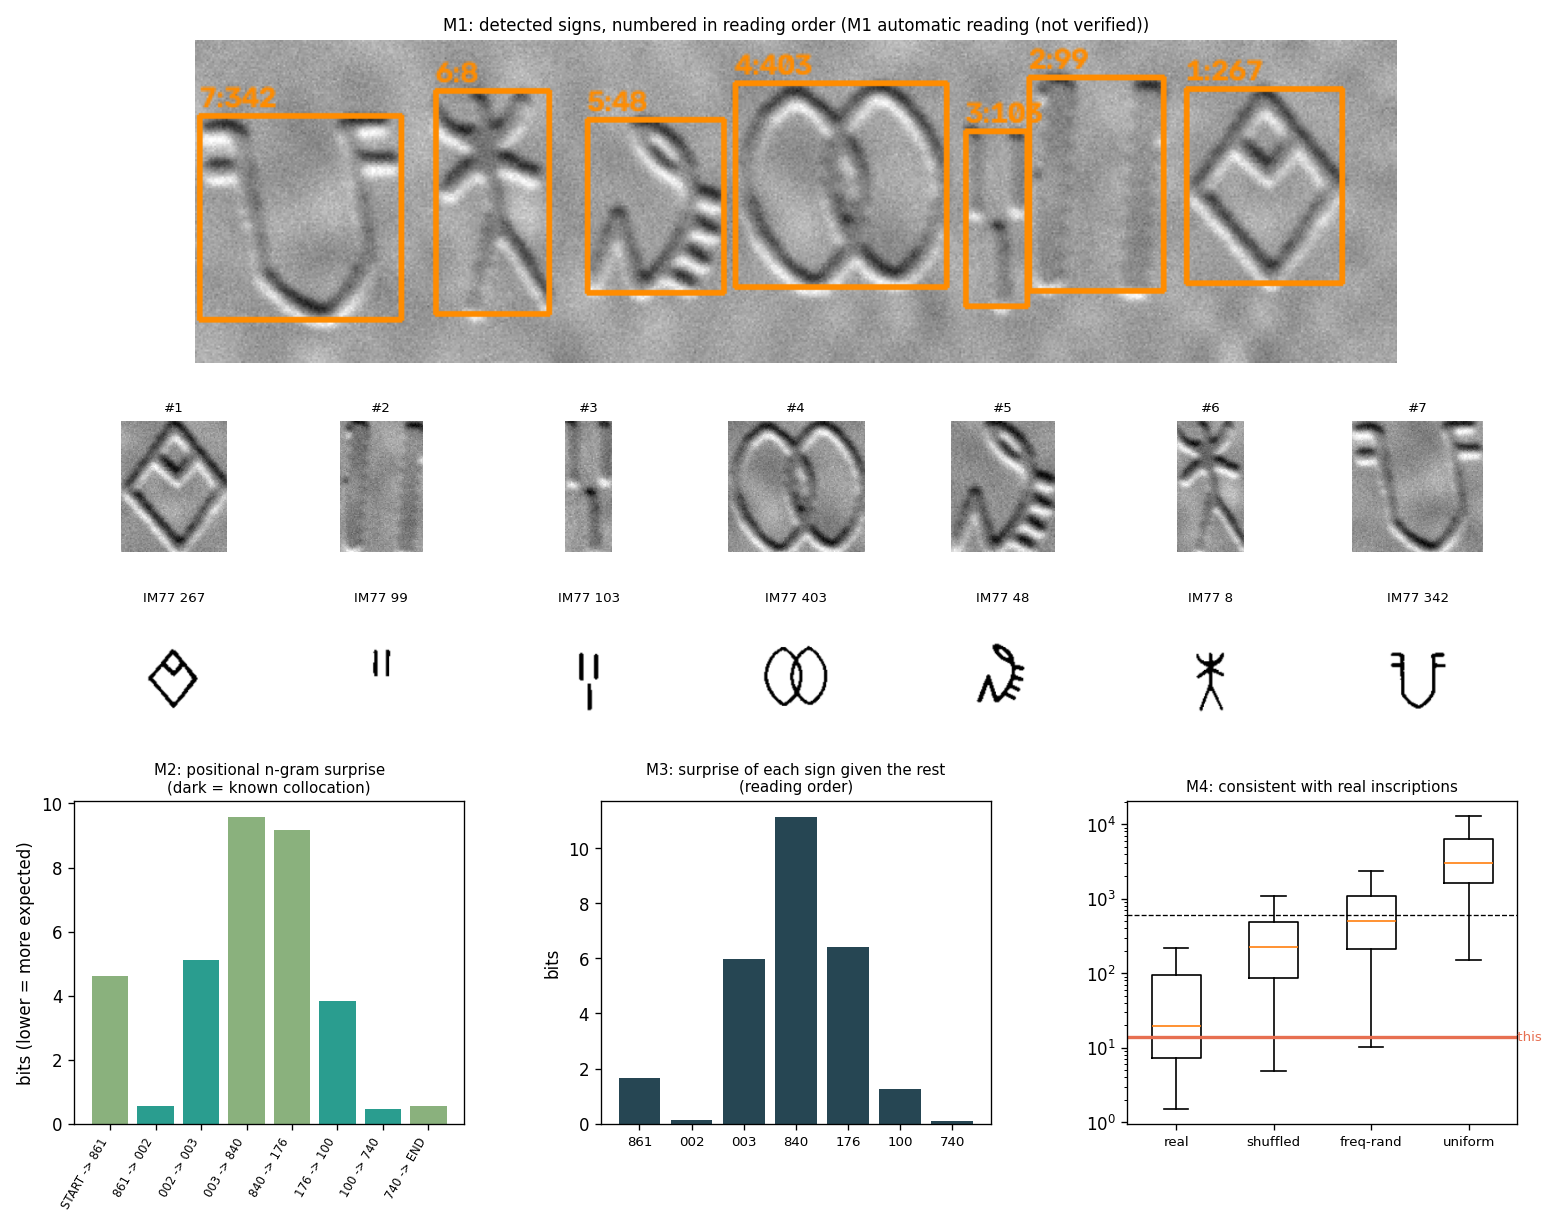
\includegraphics[width=\columnwidth]{figures/engine_panels.png}
\caption{Engine output for a held-out inscription drawn as a synthetic strip. Top: M1 boxes and IM77
IDs in reading order (right-to-left); middle: crops vs.\ templates (all 7 correct); bottom: M2
transition surprise (teal = significant collocation), M3 surprise of each sign given the rest, and the
M4 verdict (red line) against real and control distributions (dashed: threshold $\tau$).}
\label{fig:engine}
\end{figure}

\section{Experimental setup}
\textbf{Splits.} The CSV contains duplicates; we deduplicate on sign sequence (3,491 unique texts) and
split 80/10/10 (2,792/349/350) so that no sequence occurs in two splits. Signs seen fewer than twice
are mapped to unknown (426-sign vocabulary; 4.3\% of test signs unknown). M3 is evaluated by
leave-one-out masking on the test split and by 5-fold cross-validation over all 3,491 texts (12,525
predictions). \textbf{Baselines.} Unigram frequency and a bidirectional Witten--Bell bigram for M3;
four structural controls for M4. \textbf{Metrics.} Top-$k$ accuracy, perplexity (lower is better),
expected calibration error (ECE), ROC AUC, guardrail flag rate, with Wilson, bootstrap or
cross-validation intervals; McNemar's test for paired accuracy. M1 on real data is judged by hand on
two random samples of 70 detections from 77 real strips (Indus-Seal-Dataset~\cite{isd}), since no
ground truth exists. \textbf{Software/hardware.} Python 3, PyTorch 2.5, Ultralytics, scikit-learn; M1 trained on
an Apple laptop GPU (MPS), the rest on a laptop CPU.

\section{Results}
\textbf{M1.} Detection transfers to real strips; recognition does not (Table~\ref{tab:m1}). All three
of our vision models (detector, recognizer, and a relief-to-line-art U-Net that collapsed to 17 sign IDs)
scored near-perfectly on synthetic data, and no synthetic score predicted real performance.

\begin{table}[h]
\centering
\small
\begin{tabular}{lcc}
\toprule
Measure & Synthetic & Real \\
\midrule
Detector mAP50 & 0.995 & -- \\
Strips with detections & -- & 76/77 \\
Detection precision & -- & 77--86\% \\
Recognition top-1 & 87.9\% & 12--17\% \\
Recognition top-5 & 97.7\% & 40--41\% \\
Exact whole sequence & 70\% & -- \\
\bottomrule
\end{tabular}
\caption{M1 on synthetic vs.\ real images (higher is better; chance top-1 is 0.24\%). Real top-1: 95\%
Wilson intervals 6--22\% and 9--29\% for the two recognizers.}
\label{tab:m1}
\end{table}

\textbf{M2.} On CISI (153 complete texts), sign P324 ends 45\% of texts; endings are 2.4 bits more
predictable than beginnings (null maximum 1.3); flip-test JSD 0.89 vs.\ at most 0.42 under random flips
($p<10^{-4}$). Unsmoothed bigrams assign zero probability to 46\% of held-out transitions; Witten--Bell
gives held-out perplexity 40.8 vs.\ 77.3 for add-one; 41 collocations are significant. On the Wells
corpus every finding replicates (the same jar sign ends 31\% of 2,106 complete texts; JSD 0.63 vs.\
0.13), and reading order gives lower held-out perplexity in 9 of 10 folds.
The jar sign's final-position share is 68.4\% in our corpus vs.\ 69.6\% in Mahadevan's published
table~\cite{mahadevan1977}.

\begin{table}[h]
\centering
\small
\setlength{\tabcolsep}{4pt}
\begin{tabular}{lccc}
\toprule
Model & Top-1 (\%) & Top-5 & PPL \\
\midrule
Unigram frequency & 10.3\,$\pm$\,0.3 & 24.1 & 112.0 \\
Witten--Bell bigram & 32.5\,$\pm$\,1.2 & 55.2 & 31.8 \\
Transformer (single) & 32.2\,$\pm$\,0.8 & 54.1 & 32.1 \\
Ensemble of 3 & \textbf{33.3}\,$\pm$\,0.6 & \textbf{55.7} & \textbf{28.8} \\
\midrule
word2vec (SGNS) & 22.0 & 44.5 & 186 \\
LLM2Vec (scratch) & 27.6 & 47.2 & 45 \\
\bottomrule
\end{tabular}
\caption{M3 sign restoration. Top: 5-fold CV, mean\,$\pm$\,sd over folds. Bottom: held-out test split,
mean of 3 runs. Higher accuracy and lower perplexity (PPL) are better.}
\label{tab:m3}
\end{table}

\textbf{M3.} A single Transformer ties the bigram; the ensemble wins by 0.8 points of top-1 (pooled
McNemar $p=0.008$) and has lower perplexity in all 5 folds (gap 3.0, 95\% CI 2.3--3.7)
(Table~\ref{tab:m3}). Calibration is good (test ECE 0.035).


\begin{table}[h]
\centering
\small
\setlength{\tabcolsep}{3.5pt}
\begin{tabular}{lcccc}
\toprule
Test set & PPPL & Flag & AUC & High \\
\midrule
Real (held-out) & 19.6 & 6.2\% & -- & 23\% \\
Shuffled & 224 & 21.8\% & 0.85 & 10\% \\
Markov & 54.2 & 8.1\% & 0.51 & 18\% \\
Freq.-random & 504 & 44.5\% & 0.90 & 9\% \\
Unif.-random & 2995 & 93.8\% & 0.98 & 8\% \\
\midrule
M1 on real & 1454 & 74.1\% & -- & -- \\
M1 + M3 re-rank & 378 & 35.2\% & -- & -- \\
\bottomrule
\end{tabular}
\caption{M4: median Transformer pseudo-perplexity (lower = more real), perplexity-guardrail flag rate,
Naive Bayes AUC vs.\ real (0.5 = chance), share of M3 guesses rated High confidence.}
\label{tab:m4}
\end{table}

\textbf{M4.} Both models separate real text from noise (Table~\ref{tab:m4}), but
the bigram rates Markov fakes as real as real text (median 24.7 vs.\ 25.2), and Naive Bayes is at chance
on them (AUC 0.51). On uniform-random noise, 8\% of M3's guesses are still ``High'' confidence, and none
is correct. \emph{Error propagation:} injecting M1's measured error rates into clean texts lowers M3
top-1 from 34\% to 8\% and raises the flag rate from 6\% to 70\%; the direction signal M2 relies on drops
to near chance (54\% vs.\ 50\%). On M1's real readings the guardrail flags 74\% (40 of 54 scorable
strips); letting M3 re-rank M1's top-5 halves the flag rate by changing 158 signs, i.e.\ it makes the
output \emph{plausible} without any evidence that it is \emph{correct}. \emph{A proposed reading:} the
Sanskrit readings attached to 1,763 CSV inscriptions are internally systematic (the first sign predicts
the reading's first phoneme 70.8\% of the time vs.\ 18.0\% for shuffled readings, $p=0.005$), which
shows consistency of assignment, not correctness. \emph{Generation:} Gibbs samples from M3 score 18.2
(more ``real'' than real text) because M3 judges its own samples; 23\% copy a training inscription and
another 31\% are one edit away. Of the novel ones that pass the guardrail, 60 were rendered and read back:
the engine recovered 67\% of sequences exactly, yet the guardrail passed 96\% of the \emph{misread}
ones. \emph{Engine:} on 100 held-out texts drawn synthetically, 88\% of signs are read correctly.

\section{Discussion and limitations}
Three lessons recur. (1)~\emph{Synthetic validation does not predict real performance}: every vision
model scored 88--99.5\% on synthetic data and failed on carved stone. (2)~\emph{A model cannot police
its own kind}: the bigram cannot flag Markov text, M3 rates its own samples as more real than reality,
and re-ranking produces confident but unverified readings. (3)~\emph{Short texts cap what context
models add}: with five signs per text a bigram captures most of the signal. Our guardrail detects noise, not single-sign errors or meaning.
Limitations: real M1 accuracy rests on 140 hand-judged detections, and the best (17\%) recognizer's
weights were overwritten (the released one scores 12\%); near-duplicate texts remain across splits;
the threshold fixes a 5\% false-flag rate by construction; LLM2Vec was trained from scratch. Next steps: hand-annotated real seals (e.g.\ the data of
Dixit et al.~\cite{dixit2025}) and recognition restricted to the 39 frequent sign classes they use.

\section{Conclusion}
Positional structure in the Indus script is real and replicates across corpora, and a calibrated masked
model can restore about a third of damaged signs. But fluency, low perplexity and high confidence are
cheap: our own pipeline produced each of them for outputs that were wrong or meaningless, and only
controls that remove the language exposed this.

\section*{Individual member contributions}
{\small
\begin{tabularx}{\linewidth}{@{}l X@{}}
\toprule
Name & Contribution \\
\midrule
Member One & M1 vision pipeline: synthetic data, detector and recognizer training, real-strip evaluation and hand review; Sections 3--5 (M1). \\
Member Two & M2 positional and Markov analysis on CISI, smoothing validation, collocations, error-propagation simulation; Section 5 (M2). \\
Member Three & M3 masked-sign model, baselines, calibration; M4 controls, guardrails and engine integration; Sections 1--2, 6--7. \\
\bottomrule
\end{tabularx}}

\smallskip
\noindent All members have read this report and agree with the statement above.

\section*{Generative AI disclosure}
We used Claude (Anthropic; model \texttt{claude-opus-5-5}, Claude desktop app) to audit the milestone
code; write the integration code (shared modules, M2 replication, M3 de-duplication and
cross-validation, M4 experiments, engine, generation, demo, notebooks); run the experiments; and draft
this report and the documentation. We checked all such output, re-ran every reported number from the released
code, and take responsibility for it. No LLM is part of the method itself (LLM2Vec in Table~\ref{tab:m3}
is a small model trained from scratch on the sign corpus).

\section*{Code availability}
\noindent Code and data:\\
\url{\githuburl}\\
The README and \texttt{run\_all.sh} reproduce every number here; \texttt{demo/demo.py} runs the engine.

\begin{thebibliography}{99}
\small
\bibitem{russell2021aima}
S.~Russell and P.~Norvig.
\newblock \emph{Artificial Intelligence: A Modern Approach}, 4th edition.
\newblock Pearson, 2021.
\bibitem{mahadevan1977} I.~Mahadevan. \emph{The Indus Script: Texts, Concordance and Tables}. Archaeological Survey of India, 1977.
\bibitem{wells2015} B.~K.~Wells. \emph{The Archaeology and Epigraphy of Indus Writing}. Archaeopress, 2015.
\bibitem{cisi1987} J.~P.~Joshi and A.~Parpola. \emph{Corpus of Indus Seals and Inscriptions}, Vol.~1. Suomalainen Tiedeakatemia, 1987. Digital corpus: \url{https://github.com/mayig/indus-valley-script-corpus}.
\bibitem{csvsource} \textbf{[TODO: source of the Wells-numbered inscription CSV, data/raw/m3\_csv/inscriptions.csv.]}
\bibitem{im417} IM-417-150 sign images. Kaggle dataset \texttt{storesource/im-417-150}.
\bibitem{isd} Indus-Seal-Dataset (77 inscription crops). \url{https://github.com/akksshhaay/Indus-Seal-Dataset}.
\bibitem{rao2009} R.~P.~N.~Rao et al. Entropic evidence for linguistic structure in the Indus script. \emph{Science} 324(5931):1165, 2009.
\bibitem{yadav2010} N.~Yadav et al. The signs of a script: Statistical analysis of the Indus script. \emph{PLoS ONE} 5(3):e9506, 2010.
\bibitem{farmer2004} S.~Farmer, R.~Sproat and M.~Witzel. The collapse of the Indus-script thesis. \emph{Electronic Journal of Vedic Studies} 11(2), 2004.
\bibitem{sproat2014} R.~Sproat. A statistical comparison of written language and nonlinguistic symbol systems. \emph{Language} 90(2):457--481, 2014.
\bibitem{dixit2025} V.~Dixit et al. Deep learning in archiving Indus script and motif information. \emph{J.\ Computer Applications in Archaeology} 8(1):156--169, 2025.
\bibitem{wittenbell1991} I.~H.~Witten and T.~C.~Bell. The zero-frequency problem. \emph{IEEE Trans.\ Information Theory} 37(4):1085--1094, 1991.
\bibitem{devlin2019} J.~Devlin et al. BERT: Pre-training of deep bidirectional transformers for language understanding. \emph{NAACL}, 2019.
\bibitem{salazar2020} J.~Salazar et al. Masked language model scoring. \emph{ACL}, 2020.
\bibitem{guo2017} C.~Guo et al. On calibration of modern neural networks. \emph{ICML}, 2017.
\bibitem{yolov8} G.~Jocher, A.~Chaurasia and J.~Qiu. Ultralytics YOLOv8, 2023. \url{https://github.com/ultralytics/ultralytics}.
\bibitem{howard2019} A.~Howard et al. Searching for MobileNetV3. \emph{ICCV}, 2019.
\bibitem{mikolov2013} T.~Mikolov et al. Distributed representations of words and phrases and their compositionality. \emph{NeurIPS}, 2013.
\bibitem{llm2vec2024} P.~BehnamGhader et al. LLM2Vec: Large language models are secretly powerful text encoders. \emph{COLM}, 2024.
\end{thebibliography}

\end{document}
